\documentclass[a4paper, 11pt]{article}
\usepackage{graphicx}
\usepackage{amsmath}
\usepackage[pdftex]{hyperref}

% Lengths and indenting
\setlength{\textwidth}{16.5cm}
\setlength{\marginparwidth}{1.5cm}
\setlength{\parindent}{0cm}
\setlength{\parskip}{0.15cm}
\setlength{\textheight}{22cm}
\setlength{\oddsidemargin}{0cm}
\setlength{\evensidemargin}{\oddsidemargin}
\setlength{\topmargin}{0cm}
\setlength{\headheight}{0cm}
\setlength{\headsep}{0cm}

\renewcommand{\familydefault}{\sfdefault}

\title{Machine Learning 2015: Project 1 - Regression Report}
\author{mwurm@student.ethz.ch\\ ADDME@student.ethz.ch\\ ADDME@student.ethz.ch\\}
\date{\today}

\begin{document}
\maketitle

\section*{Experimental Protocol}
This is the protocol of the group "I don't care (about the name of the group)".

\section{Tools}
For our approach we used python in combination with numpy and the machine learning library "scikit-learn". Like this, python offers an API comparable to matlab, and it offers functionality, wich is very usefull for the project.

\section{Algorithm}
After trying out several algorithms we finally stick with the RandomForestEstimator of scikit-learn. Although the class of decision tree algorithms, this algorithm belongs to, has not been mentioned in the lecture yet, this class contains rather easy to understand algorithms which tend to return good results.
The used RandomForestRegressor is a perturb-and-combine techniques [B1998], what means, that it is intrinsically composed out of multiple executions of a basic algorithm. This algorithm is the decision tree algorithm in our case.
It builts a tree of decisions, which are made by using the available data. The deeper the trees become, the complexer the decision process will be, and the better the data will be fitted. By using this approach, heavy preprocessing of the data is not mandatory.

\section{Features}
First of all a MinMaxNormalization has been performed.
Concerning feature transform we added additional dimensions to the features, sothat we can perform polynomial regression. Unfortunately, adding additional degrees to all dimensions did not lead to an improved result. 
Feature selection was another important part. Given 14 dimensions, it could be estimated, that not all of them are important to get a good fitting. As indicated by its name, the \"f\_regression\" gives reason to choose it as a possible selector. It tests all regressors sequentially in a fast way to estimate the influence of the single dimensions. Then it drops all, but the k leading ones. Like this we got the best results.


\section{Parameters}
The parameter estimation is of course an important part for the random forest algorithm. Based on decision trees, the results can be unstable because small changes can end up in a completely different decision tree. To get a better overview, we first tried the method with a small set of parameters. We quickly recognized, that the sequential recompilation and execution of the test, would take an enourmous amout of time. Therefore the program has been optimized to enable a higher performance.
Scikit-learn has already all necessary features included. The included GridSearchCV function, runs a cross validation based, fitting-performance test over all combinations of possible parameters, which are given in a separate list. The cross validation makes it possible to immediatly estimate the presicion of a certain configuration. The whole process from Feature Selection, over transformation to the fitting of the regressor can be combined within a single "Pipeline". Like this, the GridSearch can not only be applied to the selection of regressor parameters, but also to the selection of the amount of interesting features.
To make it possible to search a huge grid, performance is an important issue. Due to the fact, that all grid executions are independent, parallelization is fortunately easily possible (and also supported by the scikit implementation). To take the most out of this fact, the easily accessible BRUTUS cluster of ETH, was a welcome possibility to execute the script.
\begin{figure}	
	\centering
	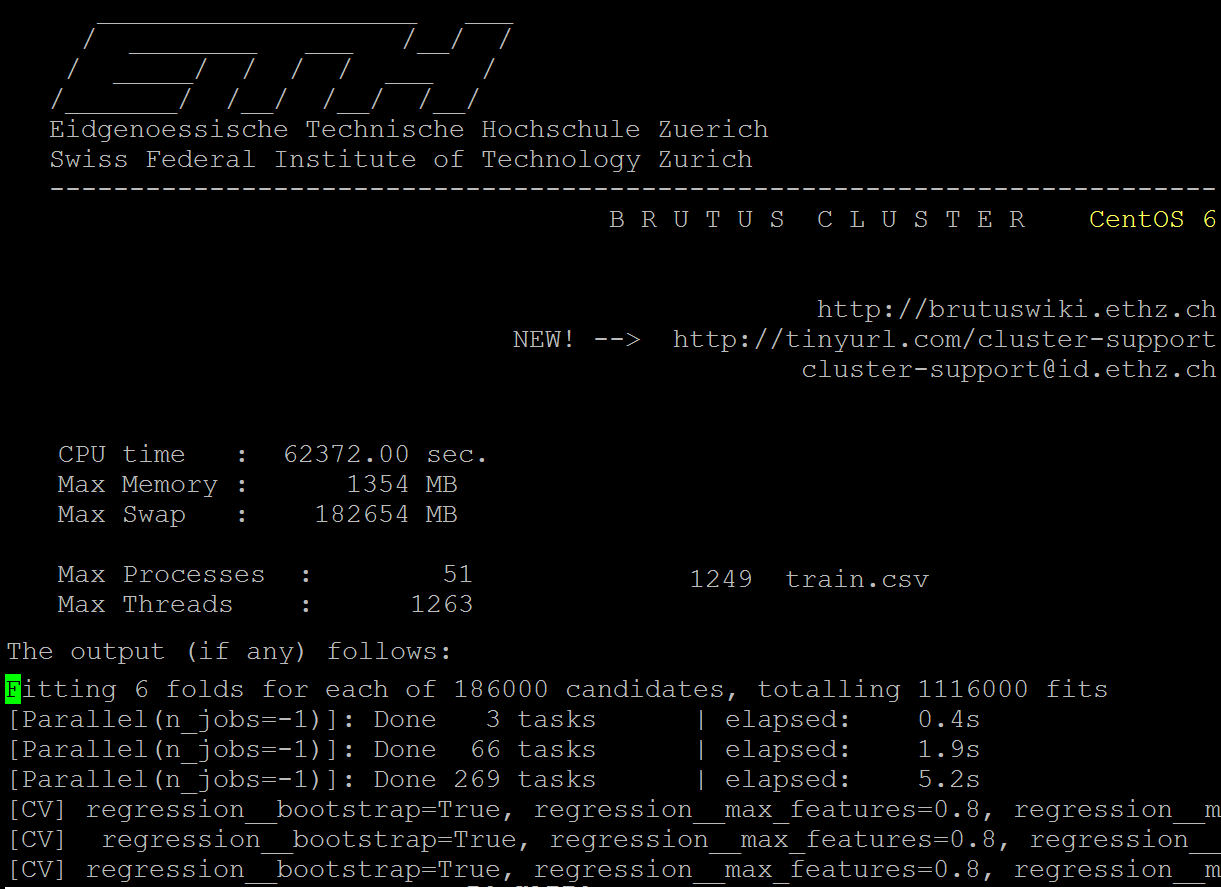
\includegraphics[scale=0.6]{ScreenshotCluster.png}
\end{figure}
The best result has been then choosen as submission.

\section{Lessons Learned}
In the beginning of the project we tried the differen linear regressors, mentioned in the lecture. The switch to the RandomForestSelector promised better results. Nevertheless we think, that in the end, the linear methods could outperfom the decision tree approach if the inherent structure of the data, would be involved stronger into the fitting process. Adding features is an important case in this situation. The given data comprises multiple dimensions, which can be seen as classes, because the values are limited to a small set of values (2,4,8). The transformation of these classes into real classes would definately result in a much better result. Unfortunately, there is not enough time to implement this.

\end{document}
